% This is a "bare-bones" thesis template file.  For examples of how to
% use a few more LaTeX features, look in the 'sample' folder.  Read
% the User Guide for documentation of the 'fsuthesis' class features.

\documentclass[11pt,expanded,copyright]{fsuthesis}

% Additional packages may be loaded here.
\usepackage{graphicx}
\usepackage{listings}
\usepackage{color}
\usepackage{hyperref}
\usepackage{pgfplots}
%\usepackage{filecontents}
%\usepackage{pgfplotstable}

\definecolor{dkgreen}{rgb}{0,0.6,0}
\definecolor{gray}{rgb}{0.5,0.5,0.5}
\definecolor{mauve}{rgb}{0.58,0,0.82}

\lstdefinestyle{cstyle} {
  language=C,
  aboveskip=3mm,
  belowskip=3mm,
  showstringspaces=false,
  columns=flexible,
  basicstyle={\small\ttfamily},
  numbers=left,
  numberstyle=\tiny\color{gray},
  keywordstyle=\color{blue},
  commentstyle=\color{dkgreen},
  stringstyle=\color{mauve},
  breaklines=true,
  breakatwhitespace=true,
  tabsize=3
}

\definecolor{dkgreen}{rgb}{0,0.6,0}
\definecolor{gray}{rgb}{0.5,0.5,0.5}
\definecolor{mauve}{rgb}{0.58,0,0.82}

\lstdefinestyle{asmstyle} {
  frame=tb,
  language={[x86masm]Assembler},
  aboveskip=3mm,
  belowskip=3mm,
  showstringspaces=false,
  columns=flexible,
  basicstyle={\small\ttfamily},
  numbers=left,
  numberstyle=\tiny\color{gray},
  keywordstyle=\color{blue},
  commentstyle=\color{dkgreen},
  stringstyle=\color{mauve},
  breaklines=true,
  breakatwhitespace=true,
  tabsize=3
}

% Adapted from Lena Herrmann at http://lenaherrmann.net/2010/05/20/javascript-syntax-highlighting-in-the-latex-listings-package

\definecolor{lightgray}{rgb}{.9,.9,.9}
\definecolor{darkgray}{rgb}{.4,.4,.4}
\definecolor{purple}{rgb}{0.65, 0.12, 0.82}

\lstdefinestyle{jsstyle} {
  keywords={typeof, new, true, false, catch, function, return, null, catch, switch, var, if, in, while, do, else, case, break},
  keywordstyle=\color{blue}\bfseries,
  ndkeywords={class, export, boolean, throw, implements, import, this},
  ndkeywordstyle=\color{darkgray}\bfseries,
  identifierstyle=\color{black},
  sensitive=false,
  numbers=left,
  comment=[l]{//},
  morecomment=[s]{/*}{*/},
  commentstyle=\color{purple}\ttfamily,
  stringstyle=\color{red}\ttfamily,
  morestring=[b]',
  morestring=[b]"
}

\title{Dynamic Slice Backsolving}
%\title{A Survey of Fuzzing and New Technique for Dynamic Analysis}
\author{Clark Wood}
\college{College of Arts and Science}
\department{Department of Computer Science} % Delete if no department
\manuscripttype{Thesis}              % [Thesis, Dissertation, Treatise]
\degree{Masters of Science}                 
\semester{Spring}                            % [Spring, Summer, Fall]
\degreeyear{2014}
\defensedate{XXXXXXX}

%\subject{My Topic}
%\keywords{keyterm1; keyterm2; keyterm3; ...}

\committeeperson{Zhi Wang}{Professor Directing Thesis}
%\committeeperson{Beauxeau D'Claune}{Committee Member}
%\committeeperson{Arlip Zarseeld}{Committee Member}

\clubpenalty=9999
\widowpenalty=9999

\begin{document}

\frontmatter
\maketitle
\makecommitteepage

%\begin{dedication}
%\end{dedication}

%\begin{acknowledgments}
%\end{acknowledgments}

\tableofcontents
%\listoftables
\listoffigures
%\listofmusex

%\begin{listofsymbols}
%\end{listofsymbols}

%\begin{listofabbrevs}
%\end{listofabbrevs}

%\begin{abstract}
%This is my abstract.
%\end{abstract}

\mainmatter

%\input chapter1

\chapter{Abstract}

Finding bugs in software is a difficult but lucrative endeavour. Fuzzing is one technique for finding bugs, particularly exploitable vulnerabilities, employed by both software companies and nation-state actors. When no source code is available, fuzzing complex programs can prove difficult, and as techniques become more sophisticated they require more resources and time. We present a technique, dynamic slice backsolving, which, to the best of our knowledge, represents a novel way to reason about not only the location of user input bytes which contribute to interesting program behavior like branching, but also the exact byte value necessary to trigger a desire branch condition. We have implemented this technique in a fuzzer, which is able to reason about large and complex user input and reliably drive program execution down new code paths to explore new portions of compiled code.
 

\chapter{Introduction}


\section{Motivation}

Fuzzing, or the feeding of manipulated input to processes to try and detect software bugs and vulnerabilities, is an integral, even required, part of the work conducted by both private-sector companies like Microsoft [Q] and Google [AM] and nation-state powers and contractors. In 2014, Pwn2Own paid out 850,000 USD to participants over two days for proof of zero-day exploitable vulnerabilities, for an average of 66,000 USD per exploit [AN]. Forbes suggests black market prices are considerably higher, peaking at over \$150,000 for modern browser exploits [AO].

\section{Problem Statement}

The software community knows that programmers write buggy software, even with debugging tools and access to source code for auditing purposes. Fuzzing, however, cannot even assume source code access, because interesting programs are not always open source. As an example, Internet Explorer, a prime exploitation target, is propietary software. Successful testing depends upon the fuzzer's ability to explore the binary and detect bugs without source code. In addition, each branch instruction in assembly language introduces two new possible paths, leading to an explosion of explorable paths as binaries grow in size and complexity. Following all or most these paths, and doing so in a timely manner, requires complex software and time-memory tradeoffs.

\section{Contributions}

In this paper, we present our analysis of existing techniques for improving fuzzers' code coverage and path exploration abilities, along with our own contributions and conclusions. We begin by exploring related work in Chapter 2, which describes current fuzzers architecture and limitations. Chapter 3 describes several fundamental techniques incorporated in most modern sophisticated fuzzers. In Chapter 4, we describe our contributions, in the form of what is, to the best of our knowledge, a new technique for black box binary fuzzing, a proof of concept fuzzer which implements the technique, and testing results. Lastly, we describe possible future work and conclusions from the experience in Chapter 5.

Our technique, dynamic slice backsolving, using dynamic taint analysis to watch user input. As user input is introduced, each byte is tracked separately and, when the program transforms or manipulates user input, those transformations are recorded. When branches which depend upon user input are reached, the recorded transformations, if possible, are reversed, backsolving for a new value of a particular byte in user input which will lead execution down a different path in the binary. After execution finishes, input test cases are mutated to reflect this new information, and a new execution test runs.

The inspiration for this technique comes mainly from "A Taint Based Approach for Smart Fuzzing", which proposes a fuzzing tool architecture, involving vulnerability detection, followed by taint analysis based upon found vulnerabilities, which drives the generation of intelligent tests. Dynamic taint analysis tracks which bytes of user input are important in the binary, and these so-called "hot bytes" are made the focus of fuzzing attempts. The paper mentions it is valuable to be able to generate backward slices of program traces. This traces can be run and analyzed by programmers. In the spirit of automation, our work not only generates backward slices based on taint propagation, but also automatically solves these traces to find new byte values. Thus, for a subset of programs, we can determine not only the exact location of user input which determines a branch condition, but also generate precise values for both branch and non-branch cases.

We have implemented this technique in a proof of concept fuzzer, stubble, which operates on x86 binaries. Stubble requires no access to source code, unlike many fuzzers utilizing symbolic execution, and automatically generates test files which exercise new paths in the input program. Program input, output, and interesting conditions like segfaults are recorded during execution, and taint propagation is recorded from user input sources to branch sinks. When a tainted branch is found, stubble automically backsolves the execution slice and generates a new test case which will drive the program down the opposite path explored in the current execution. Stubble is able to reason about hundreds of bytes of user input, for instance by performing oracle attacks on binaries which check user input against large secrets, requiring O(n) test cases to solve the secret with no previous information, where n is length of the secret. Stubble has also been parallized at the process level, allowing for an arbitrary number of independent bytes to be reasoned about concurrently. We believe dynamic slice backsolving is a reasonable complementary technique to dynamic taint analysis and symbolic execution for binary fuzzing.

\chapter{Old-Abstract}

Finding exploitable bugs in binaries is a difficult but valuable endeavour. Fuzzing, or the feeding of controlled input into processes to try and detect vulnerable conditions, is one technique used by researchers and analysts. Because many project's source code is not made unavailable to protect intellectual property, applications tested for vulnerabilities are often considered black boxes. Reasoning about the inner working of a complex application when one can only observe the relationship between input and output is hard. In fact, for some situations, like properly implemented cryptography, it is provably hard. This piles difficulties onto an already complex problem, which current research attempts to solve or reduce. Among these issues this paper focuses on:
	\begin{itemize}
		\item efficient and thorough dynamic taint analysis
		\item the path explosion problem [U], and
		\item the code coverage problem. 
	\end{itemize}
 
 Dynamic taint analysis is difficult because taint can propagate directly via assignment, or indirectly via affecting control flows which affect assignment [D], which make proper implementation tricky. The path explosion problem arises from the nature of assembly languages. Jump instructions, which may make up a decent percentage of machine instructions in programs, each multiply the total number of existing paths in a binary by two. Considering the size of binaries, this quickly leads to an un-tenably large set of possible paths to explore via conventional techniques like symbolic execution. And even if it is possible to explore all paths in a binary, analysts still need sample input which can trigger the vulnerable condition, perhaps proving that the binary is exploitable along the way. Such automated exploit generation is the subject of much research [H, I].

This work aims to reduce the severity of the latter two problems while being wary of the first during implementation. Chapter 2 explains ZZZZ, Chapter 3 AAAA etc....

Instead of trying to attain more reasonable performance by using symbolic execution less or more wisely [J], we focus instead on approximating symbolic execution by using dynamic taint analysis to drive mutation. This is possible by tracking taint at the instruction level, then backsolving from the jump to the source of taint to determine smarter ways to mutate user input and create new test cases. For instance, in the below example:


\begin{lstlisting}[style=asmstyle]
call read					;instrument read syscall
mov eax, [ebp - val]		;taint propagates from val to eax reg
inc eax						;transform eax
mul eax, 5					;transform eax
cmp eax, 42					;cmp and jmp based on tainted reg value
jnz 0x8BADC0DE
\end{lstlisting}

If we already had a test case where the value read onto the stack, after the transformations, did not equal 42, then the cmp instruction would not set the zero flag, and we would jump to the memory location 0xBADC0DE. With dynamic taint analysis in place, we see taint introduced with the read syscall, then moved into the eax register (which is subsequently tainted). After some number of transformations, perhaps zero, to the value in the eax register, we see a compare instruction, which checks eax's value against an immediate value. Then we can keep track of specific taint sources, and can record any movements or transformations, we have all the necessary information to "solve" the branch. Once we reach the tainted branch, we know that user input can affect whether we jump or not, and consequently we can backsolve to find out how to affect the branch instruction. In particular, we know the conditional jump instruction jnz depends on the Z flag in the EFLAGS register. We record whatever instruction last modified each flag in EFLAGS, so we handle the compare instruction next. Because we have kept track of taint propagation, we know we can affect the value of eax, but not 42, since it is an immediate value, so we know we need to make the value in eax equal 42. We follow the instructions that have modified the value of eax and use any appropriate operands involved with the inverse operation of the one originally performed on the value to reverse the transformations to eax's value. Finally, we notice eax originally received taint when a value was moved from memory, which was read into memory using the read syscall.

This works similarly to a constraint solver, but constraint solving appears to be a traditional bottleneck, requiring generating symbolic input, usually in a different language like LLVM intermediate representation [V] and passing execution to the constraint solver.

We propose to avoid using a constraint solver entirely, and instead backsolve completely in memory. This is easier to implement than many of the clever optimizations used by S2E and could result in speedup over symbolic execution.

Because there are a finite number of conditional jumps, all of which depend on different flags or combinations of flags in the EFLAGS register, and a finite number of instructions that modify the EFLAGS register in x86, we can create cases for all possible ways jumps are decided. We only want to prove this is possible however, so we only implement a subset and instead comment on how to implement the other comparisons.

\chapter{Fuzzing by Example}

TODO fuzzing is a large field, hope to show "fuzzing" by detailing practical examples. Techniques chapter explains a more theoretical base.

\section{TODO White vs. Gray vs. Black box}

TODO Explain white vs. black box. How gray could bleed into black because of DBI. Talk about SAGE.

\subsection{Microsoft SAGE}

Microsoft's Scalable Automatic Guided Execution, or SAGE, is an example of a white box fuzzer. Researchers at Microsoft developed SAGE to deal with large, complex programs which needed to be automatically tested for deep bugs. Microsoft considers SAGE, and whitebox fuzzing in general, so important that it requires the practice in its Security Development Lifecycle. The basic SAGE execution begins when a program to be fuzzed is first run concretely with known good input. During this run, the program is instrumented with Microsoft's AppVerifier to watch for bugs. Afterwards, SAGE receives a copy of the x86 instructions executed during this run, and symbolically executes the instructions, gathering constraints to be solved later by an SMT such as Z3. Once it has a set of these constraints, SAGE will negate each constraint in the set one by one and feed this new set to Z3. Sets that pass are ranked in descending order by the number of new instructions they reveal, and return into the start of the loop, to be executed concretely again [Q].

Because SAGE is propietary, the lack of detail about certain procedures raises questions. For instance, how does SAGE know when an instruction is new? There are a limited number of x86 instructions, which can be combined in an unlimited number of ways, which means it can be difficult to tell when a truly new instruction is executed, unless one keeps a directed cyclical graph of all explored instructions, and follows a run's progress down this graph during execution. In addition, problems integral to this work, such as code coverage and path explosion, must be addressed [Q].

SAGE uses symbolic execution, and prunes paths taken with a propietary "generational search" algorithm. This algorithm prioritizes generating new test cases (TODO does it draw on the test case reduction and expansion algorithms discussed in that one paper???). It takes a set of all constraints and tries negating each constraint independently to generate a new test case. SAGE then symbolically re-executes the constraint set using TruScan [TODO CITE] [Q]. Similarly, s2e uses QEMU for instruction set emulation, and then appears to be a strong trend in white-box fuzzing. TODO ADV/DIS?

In practice, because program termination is indeterminable, white box fuzzing could run forever. And since programs at Microsoft can easily exceed one million lines of code, with complex control flow structures, pointer manipulation, and other difficult to account for code constructs, SAGE employes several performance enhancing techniques to keep fuzzing practical and economical. Symbolically executed instructions and local constraints are cached, and unrelated constraint elimination rids the execution of contraints not related to the constraint under test. How this is determined is anyone's guess, since it is impossible to know which constraints are independent until one has explored all the code in a program. SAGE also employs a flip count limit, allowing only so many negations of a particular constraint [Q]. 

This is helpful for dealing with loops, which might evaluate or modify the same constraint many times. This technique is an example of a typical tradeoff for fuzzers. A lot of program execution time is spent in loops, but deep bugs can lurk in rarely exercised parts of a loop, so fuzzers must pick some heuristic for terminating the exploration of a loop, trading code coverage for running time.

\subsection{Grey-box Evolutionary Fuzzing}

TODO

\section{Fuzzing Web Applications}

Fuzzing is a reliable and inexpensive way to find vulnerabilities not only in compiled C/C++ programs, but also in higher level scripting languages. JavaScript, as an example, is a higher-level scripting language becoming more and more prevalent as we continue to connect ever more devices to the internet and grow individual people's connectedness. Web browsers, as a portal through which to interact with millions of users, are a common target for malware and other exploitation, and JavaScript, as the de facto client-side scripting language, offers many targets. 

Web exploits such as cross site scripting (XSS) are possible because of language functionality like the eval method, which takes an arbitrary string as an input parameter and evaluates that string as if it were JavaScript source code [AE]. The authors of "A Symbolic Execution Framework for JavaScript" wrote Kudzu because of a perceived lack of sophisticated tools for fuzzing client-side Javascript. In particular, constraint solvers at the time seemed unable to reason about JavaScript string objects, which are used in various parts of the web to represent myriad types of data, and are then parsed by custom, open-source, and propietary libraries in order to cast from a string to another data type. As an example, consider the following snippet involving eval:

\begin{lstlisting}[style=jsstyle]
// Let userInput = "2 + 2"
var str = eval(userInput); 

if (str === 4) {
	everythingDies();
	throw new Error;
}
\end{lstlisting}

In this contrived example, catastrophe occurs when user input, when executed as JavaScript, returns the value 4. Without even considering the strange casting and equality rules which JavaScript operates under, there are multiple ways for user input to throw an error, making constraint solving particularly difficult. The case where userInput = "4" is straightforward, but other cases which do not look like the String "4" or the Number 4, but evaluate to it, can also trigger the error. According to the authors, before Kudzu, string solvers were unable to reason about regular expressions, string equality, or multiple variables [AD].

While JavaScript strings, and their ubiquitous usage in client-side web programming, presented one obstacle, the sheer complexity of modern web browsers presented another. Typical browsers can open and display PDFs, play media files, and execute multiple markup and programming languages like HTML, CSS, and JavaScript to present a web page to a user. Because of this complexity, the authors decided to divide possible user interaction into two, disparate spaces: an event space and a value space. The event space contains HTML elements and their state as defined by user behavior. This would include HTML elements like radio buttons or text boxes, along with their current state, such as which radio button is currently selected, along with the state transitions for the current page, such as a user clicking one radio button, then deselecting to check boxes in order. As a rule of thumb, GUI elements which users can interact with reside in the event space. The notable exception to this is any GUI element a user types into, such as a text box. Value space contains the values for these GUI elements, along with any other text which is used as input which users or other web pages have control over [AD].

Kudzu aims to discover vulnerabilities, particularly client-side code injections, by using dynamic symbolic execution to identify constraints placed upon particular input and then solve them to generate new test cases. Dynamic symbolic execution, which mixes concrete values with choice symbolic values to optimize for speed and code coverage, is basically concolic execution. Kudzu was developed for the WebKit browser and consists of two major parts:
\begin{enumerate}
	\item GUI explorer
	\item Dynamic symbolic execution engine, which includes:
	\begin{enumerate}
		\item a constraint extractor
		\item a constraint solver
	\end{enumerate}
\end{enumerate}

The GUI explorer handles the event space by exploring all possible sequences of user-defined events at random. In order to discover event handlers, the GUI explorer relies on information from Kudzu, which instruments WebKit functions. When an HTML element which can generate an event is found, or when one of these elements in removed, Kudzu's hooks notice this and inform the GUI explorer accordingly. Symbolic execution is broken down into a custom constraint extractor, which acts upon an execution trace from a concrete execution of the program, looking for control-flow statements and whether they were taken given the appropriate values compared, and a custom constraint solver, purposefully designed to handle JavaScript objects, which receives symbolic constraints from the extractor. After the solver has reasoned about the constraints on some piece of input, a new input test case is generated and fed back into the system. Since symbolic execution is costly, Kudzu identifies when user input appears to flow to one of finitely many vulnerability sinks, such as eval or document.write. Only this user input is considered symbolically. As Kudzu runs, it takes new test cases and executes the program with a mix of symbolic and concrete variables, and checks to see whether input that flows to vulnerable sinks can result in an exploit, for instance by inserting JavaScript alerts and checking to see whether they execute [AD].

Similar to SimpIL [C], Kudzu tries to circumvent the issue of solving complicated constraints by first converting JavaScript into an intermediate language called JASIL. Strings, in particular, are parsed and partitioned into several sub types which are more uniform. For instance, one type handles strings which are semantically regular expressions, another handles strings which are the concatenation of two other strings. Although not as featureful as JavaScript strings, this IL captures a large enough number of String features to allow Kudzu to find previous unknown exploits in programs. Shortcomings include an incomplete support of String operations and JavaScript regular expressions, notably backreferences, which match a previously matched string in the regex. Although representation of strings is incomplete, Kudzu reasons well enough to find two new vulnerabilities, as well as 9 previous vulnerabilities [AD].

\section{TODO Mutation vs. Generation?}

TODO Peach Fuzzer does both, overview with pictures?

\section{TODO Local vs. Network}

Do you have access to the program you are fuzzing?

\section{TODO Difficulties and Limitations}

TODO Path explosion. Code coverage. Complex file formats which mean you create shallow errors over and over again.

TODO Limitations - one-way functions like bitwise shifts and checksums, cryptographic hashes. encryption.

TODO add code examples
%http://en.wikipedia.org/wiki/User_Datagram_Protocol#IPv4_Pseudo_Header
IDEA write c program to checksum UDP packets and say whether they pass or not, have fuzzer "correct" packets to pass arbitrary, user decided checksum.
update: probably will not work without noticeable modification, but could maybe notice the situation and reverse engineer the algorithm, then print it out or start making a lookup table?

\chapter{Related Work}

\section{Taint-based Fuzzing}

The major impetus for this work is outlined in "A Taint Based Approach for Smart Fuzzing". This paper proposes a fuzzing tool architecture, involving vulnerability detection, followed by taint analysis based upon found vulnerabilities, which drives the generation of intelligent tests. As tests are run they are checked to ensure they provide adequate code coverage, and results are carefully monitored for interesting situations like crashes [A]. The paper also serves as an excellent explanation of the current state and future of fuzzing. In particular, they suggest combining taint analysis with backward slicing. The technique discussed in this paper boils down to an attempt to automatically solve slices like those introduced in [AA], which have been derived from taint analysis as much as possible.

\section{TODO Mayhem, AEG, Exploitable Bugs}

TODO AEG [I]?

While finding bugs of any sort enhances software by providing developers the opportunity to fix problems with their programs, finding bugs that lead to exploitable conditions are of special interest. A bug is exploitable if it allows adveraries to undermine confidentiality, integrity, or availability [CITE] via avenues such as information disclosure, denial of service, or remote execution of code. Because these bugs stand alone as a separate, particularly worrying class, efforts have been made to automate the process of proving whether an identified bug is also a vulnerability which can be exploited.

Mayhem, an exploitable bug-finding system, is an attempt to address this issue by exploring state space as efficiently as possible. The authors designed Mayhem to handle path explosion by monitoring system resources and balancing the need for concurrent exploration with the resources consumed by forking and running many processes. Mayhem accomplishes through hybrid symbolic execution, a technique which heuristically combines offline and online symbolic execution. Offline symbolic execution first runs a program concretely, instrumenting the process to gather information which will then be used by a separate symbolic execution engine. Online symbolic execution, instead, tries to explore the entire program symbolically by forking new processes at branches. [H]

Mayhem improves fuzzing time performance by weaving between these two modes. It is implemented as a client-server architecture, with the client running code concretely and passing specific blocks to the server for symbolic execution. Only the server outputs results or further test cases to explore concretely. The client uses block-level dynamic taint analysis, passing control to the symbolic execution server when tainted branches or jumps are discovered. Mayhem modifies its behavior based on system memory constraints, beginning in online mode and switching to offline mode when a threshhold for memory resources is reached. Upon switching, Mayhem also saves checkpoints to save its work in an attempt to reduce exploring the same code twice. [H]

TODO Mayhem techniques

AEG required source code, where Mayhem needs access only a binary to execute. Mayhem is, however, limited to a subset of all system calls for the operating system it executes on. This is deliberate on the part of the authors, who reason that OS-wide symbolic execution introduces too much overhead. Of significance as an area of future research, Mayhem, and most other fuzzing technology explored, cannot reason about taint propagated through threading mechanisms [H].


TODO similar to Automatic patch-based exploit generation is possible: Techniques and
implications, but mine doesn't require a patch?

\section{TODO Argos: 0-Day Emulator}

http://www.few.vu.nl/argos/?page=3

\section{Checksum-Aware Fuzzing}

Much of smart fuzzing involves reasoning about constraints gathered during the execution of instrumented code. TaintScope [AB] was developed as the result of the following observation: generation-based fuzzing improves as the quality (and consequently effort) of the model to fuzz improves. This means better fuzzing is accomplished by devoting more programmer time and effort, instead of allocating more computational resources. Since a programmer's time and mental resources are valuable, so fuzzers should do for them by yielding fewer test cases that result in more interesting crashes [T].

TaintScope focuses on checksums, one where area where traditional symbolic execution-based fuzzers tend to perform poorly. Other areas, which could be interesting areas of further study, are essentially any other functions that are, in one set of assumptions or another, considered one-way. For instance, bitwise shifts, being lossy, are hard to execute symbolically, as are encryption and decryption or hashing without a precomputed table. The impetus for TaintScope's design was the desire to find deeper bugs in work like network protocols, which very early on compute checksums for integrity. Before TaintScope, fuzzing said protocols often lead to lots of worthless test cases, because they all lead to similar, shallow crashes involving failing the checksum test. Since there are far more ways to fail a checksum than to pass it, fuzzers that couldn't reason about the checksum or threw random bytes in the checksum field wasted a lot of work. Instead, TaintScope identifies likely checksum integrity checks and instruments programs to let them keep going to try and find deeper, more meaningful bugs [T].

The general method is to:

\begin{enumerate}
	\item Perform dynamic taint analysis during concrete execution
	\item Identify what could be checksum validations
	\item Run the instrumented program again, modifying ZF in EFLAGS to always "pass" the  checksum
	\item If a crash results, execute again with the checksum bytes marked symbolic
\end{enumerate}

In order to identify possible checksum validations, TaintScope assumes certain x86 branches exist to validate the results of computing checksums. With correct input, the checks leading up to these branches are always either true or false, and with incorrect input they are always the opposite. During execution TaintScope watches for these conditions, and once these conditions, and the bytes involved in them, are identified, it treats the bytes and symbolic, collecting constraints during execution. After this, TaintScope can alter the previous test case to pass the checksum. However to save work, it only spends time solving these bytes when the normal test case results in a crash. To get past shallow crashes where checksums fail it will merely hot-patch the ZF before identified "checksum-based jumps". Note this approach won't work with hashes, since one-way functions can't be easily solved with constraint solvers [T].

This general scheme is accomplished with fine-grained dynamic taint analysis, that is, taint analysis at the byte level, as opposed to a more general boolean level of taint, where perhaps user input is tainted and all non-user input is untainted. As fuzzers evolve they appear to favor more and more finely-grained taint analysis.

TaintScope implements DTA using PIN to instrument syscalls in binaries. PIN\_AddSyscallEntryFunction and PIN\_AddSyscallExitFunction are used to monitor syscalls which are known to introduce taint to a system, such as open, which might open a user-specified file, or read, which might read user-defined bytes into memory. Taint is followed as it propogates throughout data via move instructions and arithmetic instructions. TaintScope's tainting policy however, transfers taint by unioning taint values whenver they both appear in an instruction. Thus, if the policy is enforced strictly, and eax and ebx were both tainted, mov eax, ebx would regard eax as now tainted with both eax and ebx, when in reality the value of ebx has been moved into eax, removing the original taint from eax. This is one example of overtainting, which should be taken into account to achieve acceptable performance. Note also that, as of the paper, TaintScope does not take into account control-flow dependencies when tracking taint [T].

DTA is used to identify the so-called "hot bytes", which are then used as symbolic values later on, should test cases warrant further attention because of a crash or other interesting behavior. This strategy has netted TaintScope 27 new vulnerabilities across several different pieces of software, most of which operate on complicated file format specifications like PNG or PCAP files [T].

\section{Intel PIN}

Heavyweight analysis techniques, like symbolic execution or dynamic taint analysis, which operate over an entire instruction set, must account for the idiosyncracies and diverse operations supported by the architecture. By leveraging a pre-existing framework like Intel Pin [M], new software can abstract away from architecture specific details like x86 variable length instructions and avoid re-inventing the wheel.

Pin, developed by Intel Corporation and the University of Colorado, performs dynamic binary instrumentation on x86, Itanium, and ARM architectures. Pin takes an arbitrary binary to be instrumented and a user-developed dynamically linked library, and instruments the binary at runtime by inserting user defined routines or changes into the application's code.

Pin's architecture is two-fold: consisting of a virtual machine for compiling and executing code, and a code cache for storing invididual code traces. An API for developing Pintools is also provided. Pin takes apart the program one trace at a time, compiling the native executable and the instrumentation code together into the same architecture. Pin defines a trace as a linear sequence of machine code instructions, terminated by either an unconditional jump or a pre-defined number of conditional jumps. Traces, hopefully, correspond to higher level control flow structures, but are also limited in size by a pre-defined maximum number of instructions [M].

The Pin VM can be broken down into three sub-components: a just-in-time compiler which instruments the binary by hooking the appropriate routines and re-compiles into the original architecture, along with a dispatcher and an emulator. The dispatcher passes code to the code cache and executes instructions, but, because Pin resides solely in userland, certain activities which occur at a lower level of the operating system, like syscalls, cannot be captured normally. The emulator handles these cases [M].

Pin injects itself into a given binary using Ptrace to modify instructions and then trap running processes to inject code in a similar manner to how debuggers like GDB attach to processes and inject software breakpoints [AK]. Just like GDB, Pin can attach to a running process or instrument a process from the first instruction. This stands in contrast to other dynamic binary instrumentation frameworks like DynamoRIO [AL], which use LD\_PRELOAD to force a new  shared library into the process context. This noisily shifts shared libraries' memory addresses to accomodate the new, pre-loaded library, and also cannot instrument the first parts of a program before the library loading code executes [M].

Pin instruments at the trace level, JIT compiling a trace and caching it for re-use. A number of Pin optimizations revolve around the compilation phase, because testing shows Pin bottlenecks tend to concentrate around the execution of instrumented code. This is perhaps because instrumenting code involves hooking perhaps both the entrance and exit to a function, which adds two jumps. In addition, transitions between the VM and code cache require saving application state. The eflags register, for instance, must be pushed onto the stack to be read or written so that the program's original eflags is preserved. Since this register is used for all jumps, among other things, it is accessed often by both Pin and the instrumented program. Thus, Pin analyzes the liveness of each flag in eflags on a per-routine basis, and avoids saving and restoring flags which are not used by the routine as an optimization measure [M].

This research leverages Pin to instrument arbitrary binaries at the instruction and syscall levels. Code is inserted to track taint introduced by user input, and recorded separately as it propagates. When taint reaches a branch, the recorded state information is used to work backwards through lossless operations to try and reason about the location and value of bytes which affect whether the branch is taken or not.

\chapter{Techniques}

Several valuable techniques for improving fuzzers' code coverage have evolved over the years. Two, in particular, inspire this work directly: Dynamic Taint Analysis and Symbolic Execution. Dynamic Taint Analysis, or DTA, provides valuable information for guided fuzzing. Symbolic execution improves code coverage by first running a program concretely to gather constraints on a particular element, then executes the program symbolically, giving these constraints over to some kind of SMT solver [CITE] to solve for what value the element should have under certain conditions. Concolic execution, which has spawned out of the desire to use symbolic execution more wisely due to performance constraints, aims for reasonable runtimes while maintaining good code coverage. These each come with their own drawbacks, a primary one of which is the lack of automated instrumentation. Historically, any amount of symbolic execution required a programmer to directly instrument source code, leading much current research to focus on automating as much as possible.

\section{Dynamic Taint Analysis}

DTA is a form of dynamic analysis, meaning analysis occurs during execution of a program. This can be contrasted with static analysis, where a program's source code is analyzed without executing the code. The IDA Pro Disassemble [AH], which takes a compiled C binary as input and statically disassembles it to produce some flavor of assembly code, is an example of a static program analysis tool, whereas a debugger, which instruments and executes a program, allowing users to manipulate and watch the process at runtime, is an example of a dynamic analysis tool.

Developers often have an incentive to obfuscate payloads or manipulate code to make static analysis more costly, such as malware and exploit writers who don't want their products detected and reverse engineered. This merely raises the bar for attackers, since software cannot be altered to the point where it doesn't perform its original function merely to escape detection and analysis. As an example, a program that begins life encrypted must at some point use or download a secret key to decrypt itself and run. This might be incredibly difficult to find using only static analysis, but by running the program and letting it decrypt itself, then snapshotting the program's state, we can circumvent the protection entirely. Thus, program obfuscation, reverse engineering and anti-RE are cat-and-mouse games.  This is why dynamic analysis is so important, and it is an open and actively researched question whether there even exists a way to provably make a program strongly obscure [AI].

In [C], the authors summarize dynamic taint analysis and symbolic execution and attempt to formalize each technique. A formal definition for DTA requires a formal language upon which to perform taint analysis, so the authors use SimpIL, a Simple Intermediate Language. Note that this is distinct from but related to the intermediate representations which some fuzzing research converts sources into. When fuzzers first convert to an intermediate language, this is done to simplify future analysis, as when Kudzu [AD] converts JavaScript strings into one of several new data types which are easier to reason about. Time is traded up front in order to make future operations easier or possible. SimpIL is a complete programming language, lacking in features but used as a base for some of the author's other work. It should be noted that the features SimpIL lacks, in particular functions and variable scoping, can be implemented using SimpIL, and SimpIL expressions not having side effects similarly do not hinder it. The important implementation issues for DTA spring from one's tainting policy. Our tainting policy decides under what circumstances we introduce taint, verify it, and track its propagation throughout the program execution [C]. Introduction rules should specify:
\begin{itemize}
	\item when taint first appears in a program,
	\item what type of taint it is, and 
	\item what parts of the program have become tainted as a result
\end{itemize}

We can record taint at varying levels of granularity, with the tradeoff of finer-grained taint requiring greater system resources and slowing down analysis. Different types of taint may be more interesting to different kinds of fuzzers because different input comes from sources of varying trustedness [C]. For instance, we should probably trust raw, unsanitized user input we have read less than we trust a configuration file that only privileged users can modify. Both might be read in as input to a program, but the former is much more likely to contain malicious data like shellcode trying to exploit a vulnerability. Fuzzers have continued to drill down into finer and finer levels of granularity, from assigning everything with a generic binary value of tainted/not tainted to byte and even bit-level marking of which part of user input affected which variable. [CITE] [C] Note that this also expands taint's data type from a bit to something larger, and each tainted object requires this tag.

Just as with taint introduction, we verify taint based on our overall objective. If we are worried about a binary being exploited to execute arbitrary code, we may instrument the EIP register. When we verify that taint has reached EIP, we know we stand a strong chance of having found an exploitable condition. Likewise, were we monitoring taint not in order to generate test cases for fuzzing, but to study a piece of malware, we might instead watch for when a particular routine, which we think is unpacking the malware, has finished, and the malware is now available in an unobfuscated form.

Taint propagates through a program from its initial source, perhaps making its way to vulnerable sinks. The condition we are interested in is when user input finds its way to these vulnerable sinks in a program, and is able to influence them. As an example, user input received on STDIN which is able to change the value of the EIP register in x86 assembly is able to hijack control flow in the program. This may be as innocuous, though annoying, as forcing EIP to strange areas in the binary, resulting in segfaults, to more sinister remote code execution via pointing EIP to user controlled shellcode.

There are several challenges involved with implementing DTA. First of all, accurate taint analysis, as free as possible from both over and under tainting, requires a precisely implemented taint policy. Different types of control flows, either direct or indirect, must be handled as well, and one-way or lossy functions also tend to be either difficult or untenable to instrument.

[C] suggests that taint introduction is an easier problem than taint removal. After all, taint is introduced into a system by a limited number of avenues, such as files, user input, and the execution environment. Once these are instrumented, they can be considered as always introducing taint to the system. However, taint removal depends not only on the instruction execution, but also on the context of the instruction. In x86, performing the exclusive or operation with the same register as both operands will zero out the register. Thus, even if the eax register were tainted, after xor eax, eax the eax register will be untainted, as its value is always 0. Taint policy could, for instance, add a rule that xoring a register with itself will remove taint from the register. However, what if eax and ebx are both tainted with the same value and we execute xor eax, ebx? Now the check must not just blindly remove taint when the same register is both operands, but instead consider the source of taint found in both operands. Failing to account for circumstances like this introduces overtaint, which means we spend time analyzing false positives. 

Even worse is undertainting. Overtainting creates unnecessary work, but undertainting may lead us to miss taint propagations to vulnerable sinks. Undertainting typically occurs when we mishandle or fail to perceive information flows [C]. Taint can propagate via explicit or implicit flows, sometimes also called data and control dependencies respectively [G]. Explicit flows involve a tainted variable, x, which is used in an assignment expression to compute a new variable, y. In this situation, x taints y, and if y is involved in any further assignment to a variable z, then x taints z by transitivity. In contrast, implicit data flows involve a tainted variable used to affect control flow within a program which subsequently sets the value of another variable, for instance at a branch [D]. 

Handling taint correctly is of great importance because of the existence of subtle implicit flow cases referenced by Clause, J. et al [D]. Implicit data flows are not always considered by dynamic tainting techniques [E], but for my project, implicit data flows are very important, so we need to implement DTA which catches both implicit and explicit flows.

TODO Finish brumley DTA
TODO undertaint info flow code example

TODO one-way functs
Use: https://www.ida.liu.se/~TDDC90/literature/papers/violating05.pdf
[AJ]


DTA has been used to implement smart mutation fuzzers [A, T, MORE], but we believe the technique we explore later is unique from and complementary to Bekrar's work. In [A], DTA is proposed as a way to intelligently decide which parts of user input should be mutated. In [T], dynamic taint analysis identified hot bytes, which were then modified randomly or with boundary values. We plan to add on to these ideas by allowing smarter mutations to be selected by backsolving to decide which values are most likely to result in new paths being explored. This has been done with symbolic execution before, but traditional symbolic execution is much more heavy-weight, both in time required to setup the environment and in overhead introduced to run the program, than my proposed approach.

\section{Symbolic Execution}

TODO Add "All you ever wanted to know..." Stuff
TODO more stuff from O

Symbolic execution supplies symbolic instead of concrete values for input [O]. This technique has been used to effectively detect bugs in software [Q], although historically it has required access to source code, which makes traditional symbolic execution infeasible in many vulnerability research situations where source code is unavailable. In addition, symbolic execution often uses instruction translators like QEMU [K] and satisfiability modulo theorem solvers like Z3 [P], which introduce significant overhead. This makes it difficult for symbolic execution to scale past the order of tens of thousands of lines of code. 

Symbolic execution is defined under SimpIL as execution under which return values from input sources are symbolic, instead of concrete. As the program executes, we pick up various constraints on these symbols from expressions and branches. For instance, we may start with a symbol s, which is then multiplied by a scalar 10, and then added to a constant 5 to calculate the offset for an effective address in an array. The symbol s is now constrained as s*10+5. When we encounter branch instructions, we inherit constraints based on whether or not the branch is taken. If we branch in the figure below, we now have the constraints x * 10 + 5 == 25 [C].

\begin{lstlisting}[style=cstyle]
s = get_input();
index = s * 10 + 5;
if A[index] == 25
	func1();
else
	func2();
\end{lstlisting}

Because symbolic execution can reason about the constraints placed on input, it drastically reduces the amount of testing necessary to explore all possible branches [C]. With purely random testing in the above example, we would need to provide many different values for s to trigger the if statement and explore func1. If fact, only one value, s = 2, leads us down this path, where all other values jump to func2. Just for integer based evaluations, we would need to test half of all integer values to stand a reasonable chance at triggering both paths of any if statement. Symbolic execution, in contrast, solves for s = 2 and s $\neq$ 2, requiring only two separate executions to explore both paths. However, this precision comes at a cost. Symbolic execution doubles the number of paths which must be explored each time we encounter a  branch, since we can either take or not take each branch. Most optimizations for symbolic execution boil down to using symbolic execution less, parallelzing symbolic execution, or trying to simplify constraint formulas to make them easier to reason about [C]. Using symbolic execution less or more smartly falls into the realm of concolic and mixed execution. Parallelization introduces its own set of challenges, raised in [H], such as efficiently using resources by controlling the number of forked programs executing.

Not only is symbolic execution costly, but certain things are difficult to reason about symbolically. Accessing memory, for example, is hard to do when we reference not a memory location but an unevaluated expression. Solutions to this are imperfect and tend to rely on a combination of outsourcing the work to an SMT solver and performing static analysis on the binary to try and guess about memory locations. Schwartz, Avgerinos and Brumley raise the concern that malware could take advantage of most symbolic execution engines inability to perfectly reason about symbolic memory to frustrate malware analysts [C].

Certain constructs, like switch statements, when translated into assembly, are converted into jump tables, which consist of a sequence of checks and jumps to implement each case. During symbolic execution these compares and jumps could also be an expression instead of a concrete value. Syscalls and operations involving I/O are also difficult to express in a purely symbolic execution, because they can have side effects. For example, the write syscall not only returns an integer value representing success and number of bytes written, but also writes to a file descriptor. Implementation can model this effect to an external entity, but because of the unique side effects each syscall have, there will be many one-offs [C]. 

Without utilizing symbolic execution, however, it is difficult to automatically guarantee that all possible paths in a binary have been explored. Where most current research focuses on improving speed by using symbolic execution less, we propose to achieve similar code coverage to symbolic execution by implementing something akin to symbolic execution, but without using the SMT solvers and instruction emulation which tend to make symbolic execution slow.

Call-chain-backward symbolic execution has been proposed by [R], although this technique achieved a backward symbolic execution by iteratively applying a forward execution from successively farther away points in the program and the reducing the set of possible symbolic inputs. In contrast, we propose to avoid symbolic execution, forward or backward, by backsolving concretely and then applying heuristics to generate concrete input which is highly likely to result in exploring a new path. Symbolic execution never occurs, although we believe in many situations an equal degree of precision in determining new paths can be attained.

\section{Mixed and Concolic Execution}

TODO TODO TODO [C] considers concolic execution to be when we first execute concretely and THEN execute the same thing symbolically. Mixed execution is when we execute once with both concrete and symbolic input--make sure other works stand by this distinction.

TODO talk about how this is called many different things, and is a rather amorphous term.

Current research focuses on carefully deciding when and how to use symbolic execution [J, T, W]. So-called concolic execution mixes concrete and symbolic input, and various heuristics to determine when to resort to symbolic execution are in research.

Concolic testing has been shown to improve runtime while still allowing both wide and deep inspection of a program's execution tree, although it often still requires source code to be instrumented [X, Y]. What We propose is similar to concolic testing, in that we are augmenting concrete execution with dynamic taint analysis to solve for mutations which will exercise new paths in the code. However, the lack of a heavyweight constraint solver and the ability to work on binaries without instrumenting or using source code in any way have, to the best of my knowledge, not yet been proposed.

Koushik Sen defines concolic testing as combining "random tesing and symbolic execution to partly remove the limitations of random testing and symbolic execution based testing" [AB]. This differs from hybrid symbolic execution engines like Mayhem [H], which switch between different types of symbolic execution. Hybrid symbolic execution does not itself supplement fuzzing by adding concrete random values. Both imply a tradeoff between two types of analysis, however, and thus both, when implemented by different people, will differ in where they assign the tradeoff. Some concolic testing, for instance, will start with concrete values which are random, or NULLs for pointer values. After an execution, one of the symbolic constraints will be negated, to allow a new path to be explored, and the program will be run again with new random input [AB]. Various research aims to either use symbolic execution less [Q, R, X], pick better than random values [A], or pick better input bytes to give random values [A, E, T, AB].

\section{TODO Conversion to an Intermediate Representation}

Used in javascript fuzzer [AD]
Used in [C].
Mitigates dealing with side effects, done by PANDA.
%http://www.cc.gatech.edu/~brendan/tzb_author.pdf
%http://iris.lib.neu.edu/cgi/viewcontent.cgi?article=1097&context=elec_comp_theses

\chapter{Contribution}

We have implemented a proof of concept fuzzer which uses dynamic taint analysis to record the operations performed on user input, then reverses these operations to solve for new paths to explore. The fuzzer currently records implicit and explicit taint flows between memory and registers. When the EFLAGS register is modified, it is checked whether a comparison instruction with tainted operands was the modifier, and if so this is also recorded. After an execution it publishes input, output, taint, and mutation data to a driver program, which reasons about possible user input locations and values one byte at a time. This means when branch decisions are determined by comparisons at the byte level, the fuzzer can guarantee a new path is taken, provided it can accurately backsolve information about the transformations performed on the byte.

\section{Assumptions and Scoping}

We assume ASLR is disabled for the binary to be fuzzed. This allows the program to easily track and compare execution paths. We have implemented the technique for the x86-32 architecture, because x86 is widespread, and vulnerabilities resulting from unsafe C code should persist across binaries, regardless of both the size and flavor of architecture (32 vs. 64-bit, ARM vs. x86 vs. PowerPC etc.), since compilers try to adhere to the C standard and vulnerabilities like buffer overflows exist at a C source code level. We also assume the presence of an algorithm which will detect an exploitable condition, provided it is given the proper binary and input to the binary, and an initial test case. The program concretely executes the binary once with the initial test case, recording taint propagation during execution. Stdin, stdout, and stderr are recorded for each run, for later analysis. After the initial run, the program automatically starts solving each byte by backsolving to try and find new paths.

TODO in above make sure can catch stderr segfaults, segfaults go to shell's stderr, also a signal

Current selective symbolic execution engines still appear to introduce significant overhead, between 6 and 78X overhead more than QEMU for S2E. Just QEMU is between 4 and 10 times slower on some benchmarks, closer to 15 on others [J, K, L]. In contrast, basic block counting using Intel Pin, the framework we are leveraging, introduced between 2 and 4X overhead [M]. However, the pintool needed for my proposed technique introduces greater levels of overhead, since we will be working at the instruction level instead of the basic block level, requiring more insertions for any given binary.

We are leveraging Intel PIN to perform dynamic binary instrumentation. We are testing dummy programs with many paths that are easy to backsolve, similar to the example above. A C program which uses sequential switch statements to check user input against a secret, when compiled with tcc, which performs very little optimization, is such an example binary. 

There are allowable situations in programs which are outside the scope of this program. For instance, programs can loop forever [X]. These can be dealt with using reasonable heuristics, fuzzers tend to simply count loops and terminate after a set threshold is reached, and could be the subject of future research.

% TODO We then plan to test against S2E and Peach Fuzzer [Z]. 

\section{Implementation}

We implement dynamic taint analysis for files as input sources. We are basing my implementation of DTA on Jonathan Salwan\'s work [N]. Currently we instrument the read syscall, watching for all reads executed, then tag user input at the byte level and follow it as it moves throughout the binary. We instrument binaries at the assembly instruction level using Intel Pin, which dynamically disassembles each instruction. Each instruction is handled differently based upon the following criteria:

\begin{itemize}
	\item Is the instruction a conditional jump?
	\item Is the first operand a memory location or a register?
	\item Is the first operand read or written?
	\item Is the first (second if applicable) operand tainted?
\end{itemize}
	
For example, move operations involving an untainted first operand and a tainted second operand generally spread taint, while those with a tainted first operand and an untainted second operand remove taint. Tainted branches trigger the backsolving technique. Various precautions, such as removing taint for an instruction like "xor eax, eax", must be taken. Lossy operations, like shifts, must be handled carefully to be backsolve-able, and checksums and cryptographic operations are not supported.
	
As a demonstration we have run our fuzzer, Stubble, against various binaries which open a file and check specific bytes in a file for specific character values. If all of these checks pass, then the program outputs a "win" string, otherwise it outputs a "lose" string. This can be thought of conceptually as an oracle attack, and is similar to reverse engineering "crackme" exercises. Given no knowledge of the secret key, and only able to query an oracle, a successful attack must discover the secret within a reasonable number of guess [CITE?].

After compiling with the Tiny C Compiler, which performs minimal optimization and doesn't add security measures, this binary and a default test file are given as input to Stubble, which will begin to dynamically generate run cases which will explore new paths within the binary. These test cases are fed back into the system, which continues to backsolve to find new ways to explore at branches, until there are no tainted bytes left for exploration.


% (segfault? EIP? add vulnerability detection alg?). We have observed .... (insert graphs with password lengths, etc.)
	
\section{Results}

Secrets of length 1 to 50 were tested at various intervals. It appears that, aside from some constant overhead, that test cases generated and time required to crack the binary  rise linearly with password length. The constant overhead is probably introduced from overtaint.


(TODO time smaller oracle attacks)
TODO attacks which transform input first to show ability to backsolve

\begin{figure}
\caption{Fig. 1}
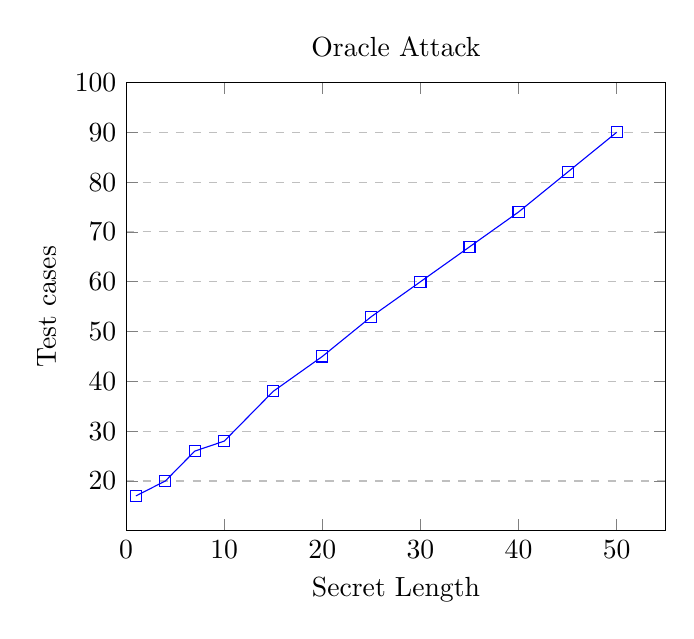
\begin{tikzpicture}
\begin{axis}[
    title={Oracle Attack},
    xlabel={Secret Length},
    ylabel={Test cases},
    xmin=0, xmax=55,
    ymin=10, ymax=100,
    xtick={0,10,20,30,40,50},
    ytick={20,30,40,50,60,70,80,90,100},
    ymajorgrids=true,
    grid style=dashed,
]
 
\addplot[
    color=blue,
    mark=square,
    ]
    coordinates {
    		(1,17)
    		(4,20)
    		(7,26)
    		(10,28)
    		(15,38)
    		(20, 45)
    		(25, 53) % 1:41.22elapsed
    		(30, 60) % 1:51.78elapsed
    		(35, 67) % 2:09.49elapsed
    		(40, 74) % 2:19.83elapsed
    		(45, 82) % 2:36.96elapsed
    		(50, 90) % 2:51.77elapsed
    }; 
\end{axis}
\end{tikzpicture}

\end{figure}

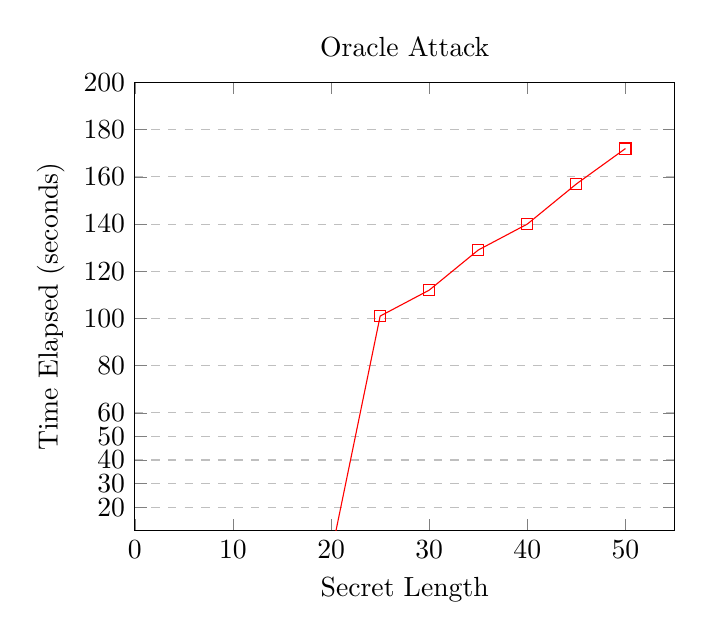
\begin{tikzpicture}
\begin{axis}[
    title={Oracle Attack},
    xlabel={Secret Length},
    ylabel={Time Elapsed (seconds)},
    xmin=0, xmax=55,
    ymin=10, ymax=200,
    xtick={0,10,20,30,40,50},
    ytick={0,20,30,40,50,60,80,100,120,140,160,180,200},
    ymajorgrids=true,
    grid style=dashed,
]
 
\addplot[
    color=red,
    mark=square,
    ]
    coordinates {
    		(1,0) % TODO time these first couple
    		(4,0)
    		(7,0)
    		(10,0)
    		(15,0)
    		(20, 0)
    		(25, 101) 
    		(30, 112)
    		(35, 129) 
    		(40, 140)
    		(45, 157) 
    		(50, 172) 
    }; 
\end{axis}
\end{tikzpicture}
	
	
\section{Testing Harness}

Fuzzers require intuitive but powerful test harnesses, so that users can easily control how a binary is fuzzed and understand the results of fuzz testing. Currently, stubble records input, output, taint for each test executed, appending an auto-incrementing id to log files and separating results at the directory level. Stubble also keeps track of the mutations which have already been explored. A driver program keeps track of the observed taint which has already been explored, and selects a new byte to mutate. Users can grep for interesting conditions like segfaults or unexpected output, then cross reference the test number with the observed taint flow, input file, particular mutation tested.

%Professional fuzzing products, like Peach Fuzzer

%\section{Methodology}

%We are currently instrumenting dummy programs which use a subset of all possible comparisons and arithmetic operations on tainted variables. If results appear promising we can try to make the fuzzer as complete as possible and begin running it on real-world applications. Achieving a noticeable speedup over modern symbolic execution would be the goal.

%As of this writing we are moving towards fuzzing Linux utilities. Results for toy binaries are promising, with "crackme" type programs which ask for a secret being solved in approximately 2*n runs, where n is the length of the secret. There is, however, still some overtainting which must be accounted for.	
%\section{Evaluation}

\section{Parallelization}

We have implemented a parallel version of the pintool, mp.c, to fork and exec a user-specified number of processes. Because a tainted branch may only be reachable based upon previous branches taken, and also because of complex conditions involving loops, the problem is not embarassingly parallel. Results show an expected speedup for an application with decently independent input.

Sequential:
After several runs, I've seen performance ranging from ~33 seconds to 19 seconds.
26.12user 7.15system 0:33.42elapsed 99\%CPU (0avgtext+0avgdata 12964maxresident)k
0inputs+1496outputs (0major+1168365minor)pagefaults 0swaps

14.66user 4.67system 0:19.44elapsed 99\%CPU (0avgtext+0avgdata 12964maxresident)k
0inputs+1496outputs (0major+1168305minor)pagefaults 0swaps

Parallel:
The parallel implementation seems to decrease time by somewhere around half, which makes sense considering the problem is not embarassingly parellel, and Intel Pin may try and use multiple cores during startup.
30.64user 9.71system 0:10.83elapsed 372\%CPU (0avgtext+0avgdata 12952maxresident)k
0inputs+816outputs (0major+1368622minor)pagefaults 0swaps

However, we have seen runs as high as ~13 seconds elapsed. Since my testing environment has 4GB ram and 4 virtual cores, 4 processes seems to give me the best speedup. We also tested with 2, 8, and 16 processes but didn't see a comparable speedup.

%
%Currently have results for crackmes, give idea of my fuzzer vs. %peach fuzz, and where i plan to go. 

\section{Lessons Learned}

TODO overtainting, naive implementations had lots of it.
TODO difficulties with implementation

\chapter{References}

\begin{itemize}
	\item [A] Bekrar, Sofia, et al. "A taint based approach for smart fuzzing." Software Testing, Verification and Validation (ICST), 2012 IEEE Fifth International Conference on. IEEE, 2012.
	\item [B] DeMott, J., Enbody, R., and Punch, W. "Revolutionizing the Field of Grey-box Attack Surface Testing with Evolutionary Fuzzing", BlackHat and Defcon 2007.
	\item [C] Schwartz, E.J., Avgerinos, T., Brumley, D. "All You Ever Wanted to Know About Dynamic Taint Analysis and Forward Symbolic Execution (but might have been afraid to ask)." 2010 IEEE Symposium on Security and Privacy.
	\item [D] Clause, J. Li, W., Orso, A. "Dytan: a generic dynamic taint analysis framework". 2007 Int'l symposium on Software testing and analysis. ACM, 2007.
	\item [E] Ajit, Beng Heng Ng Earlence Fernandes, Aluri Atul Prakash, and David Rodriguez Velazquez Zijiang Yang. "Beyond Instruction Level Taint Propagation." (2013).
	\item [F] Yamaguchi, Fabian, Felix Lindner, and Konrad Rieck. "Vulnerability extrapolation: assisted discovery of vulnerabilities using machine learning." Proceedings of the 5th USENIX conference on Offensive technologies. USENIX Association, 2011.
	\item [G] Bao, Tao, et al. "Strict control dependence and its effect on dynamic information flow analyses." Proceedings of the 19th international symposium on Software testing and analysis. ACM, 2010.
	\item [H] Cha, Sang Kil, et al. "Unleashing mayhem on binary code." Security and Privacy (SP), 2012 IEEE Symposium on. IEEE, 2012.
	\item [I] Avgerinos, Thanassis, et al. "AEG: Automatic Exploit Generation." NDSS. Vol. 11. 2011.
	\item [J] Chipounov, Vitaly, Volodymyr Kuznetsov, and George Candea. "S2E: A platform for in-vivo multi-path analysis of software systems." ACM SIGARCH Computer Architecture News 39.1 (2011): 265-278.
	\item [K] Bellard, Fabrice. "QEMU, a Fast and Portable Dynamic Translator." USENIX Annual Technical Conference, FREENIX Track. 2005.
	\item [L] Guillon, Christophe. "Program Instrumentation with QEMU." 1st International QEMU Users’ Forum. 2011.
	\item [M] Luk, Chi-Keung, et al. "Pin: building customized program analysis tools with dynamic instrumentation." Acm Sigplan Notices. Vol. 40. No. 6. ACM, 2005.
	\item [N] Salwan, Jonathan. Shell-storm.org http://shell-storm.org/blog/Taint-analysis-and-pattern-matching-with-Pin/
	\item [O] King, James C. "Symbolic execution and program testing." Communications of the ACM 19.7 (1976): 385-394.
	\item [P] De Moura, Leonardo, and Nikolaj Bjørner. "Z3: An efficient SMT solver." Tools and Algorithms for the Construction and Analysis of Systems. Springer Berlin Heidelberg, 2008. 337-340.
	\item [Q] Godefroid, Patrice, Michael Y. Levin, and David Molnar. "Sage: Whitebox fuzzing for security testing." Queue 10.1 (2012): 20.
	\item [R] Ma, Kin-Keung, et al. "Directed symbolic execution." Static Analysis. Springer Berlin Heidelberg, 2011. 95-111.
	\item [S] Boyer, Robert S., Bernard Elspas, and Karl N. Levitt. "SELECT—a formal system for testing and debugging programs by symbolic execution." ACM SigPlan Notices. Vol. 10. No. 6. ACM, 1975.
	\item [T] Wang, Tielei, et al. "Checksum-aware fuzzing combined with dynamic taint analysis and symbolic execution." ACM Transactions on Information and System Security (TISSEC) 14.2 (2011): 15.
	\item [U] Cadar, Cristian, and Koushik Sen. "Symbolic execution for software testing: three decades later." Communications of the ACM 56.2 (2013): 82-90.
	\item [V] Cadar, Cristian, Daniel Dunbar, and Dawson R. Engler. "KLEE: Unassisted and Automatic Generation of High-Coverage Tests for Complex Systems Programs." OSDI. Vol. 8. 2008.
	\item [W] McCamant, Stephen, et al. Transformation-aware symbolic execution for system test generation. Tech. Rep. UCB/EECS-2013-125, University of California, Berkeley (Jun 2013), 2013.
	\item [X] Majumdar, Rupak, and Koushik Sen. "Hybrid concolic testing." Software Engineering, 2007. ICSE 2007. 29th International Conference on. IEEE, 2007.
	\item [Y] Sen, Koushik, Darko Marinov, and Gul Agha. CUTE: a concolic unit testing engine for C. Vol. 30. No. 5. ACM, 2005.
	\item [Z] Eddington, Michael. "Peach fuzzing platform." Peach Fuzzer (2011).
	\item [AA] Zhang, Xiangyu, Rajiv Gupta, and Youtao Zhang. "Precise dynamic slicing algorithms." Software Engineering, 2003. Proceedings. 25th International Conference on. IEEE, 2003.
	\item [AB] Wang, Tielei, et al. "TaintScope: A checksum-aware directed fuzzing tool for automatic software vulnerability detection." Security and Privacy (SP), 2010 IEEE Symposium on. IEEE, 2010.
	\item [AC] Sen, Koushik. "Concolic testing." Proceedings of the twenty-second IEEE/ACM international conference on Automated software engineering. ACM, 2007.
	\item [AD] Saxena, Prateek, et al. "A symbolic execution framework for javascript." Security and Privacy (SP), 2010 IEEE Symposium on. IEEE, 2010.
	\item [AE] Mozilla Developer Network. https://developer.mozilla.org/en-US/docs/Web/JavaScript/Reference/Global\_Objects/eval
	\item [AF] The WebKit Open Source Project. http://www.webkit.org/
	\item [AG] Portokalidis, Georgios, Asia Slowinska, and Herbert Bos. "Argos: an emulator for fingerprinting zero-day attacks for advertised honeypots with automatic signature generation." ACM SIGOPS Operating Systems Review. Vol. 40. No. 4. ACM, 2006.
	\item [AH] Rescue, Data. "IDA Pro Disassembler." 2006-10-20). http://www. datarescue. com/idabase.
	\item [AI] Garg, Sanjam, et al. "Candidate indistinguishability obfuscation and functional encryption for all circuits." Foundations of Computer Science (FOCS), 2013 IEEE 54th Annual Symposium on. IEEE, 2013.
	\item [AJ] Oehlert, Peter. "Violating assumptions with fuzzing." Security \& Privacy, IEEE 3.2 (2005): 58-62.
	\item [AK] Gilmore, John, and Sten Shebs. "GDB internals—a guide to the internals of the GNU debugger." Found in the doc directory of gdb distribution version 5.1 (2000).
	\item [AL] Bruening, Derek, and Qin Zhao. "DynamoRIO."	
	\item [AM] http://googleonlinesecurity.blogspot.com/2011/08/fuzzing-at-scale.html
	\item [AN] http://www.pwn2own.com/, http://www.pwn2own.com/2014/03/pwn2own-2014-lineup/
	\item [AO] http://www.forbes.com/sites/andygreenberg/2012/03/23/shopping-for-zero-days-an-price-list-for-hackers-secret-software-exploits/
	

\end{itemize}


%\input chapter2
%\input chapter3

%\appendix
%\input appendix1

% You have your choice of bibliography sections, either
% hand-crafted or BibTeX.

% This is the "hand-crafted" bibliography/references section:
%\begin{references}
%Mybib, Sample. \textit{An Example of a Bibliographic Entry
% Created Manually}. Tallahassee, Florida: Fornish and Frak, 2010.

%Smith, Marigold. \textit{Lots and Lots of Bibliographic Entries
% and How to Display Them}. Tallahassee, Florida: Gibson and %Goulash, 2010.
%\end{references}

% Or use the BibTeX bibliography/references section below.  View the
% file 'myrefs.bib' to get a feel for what these entries may look
% like.  See the document in the 'sample' folder for more citation and
% BibTeX examples.

% \bibliographystyle{plain}
% \bibliography{myrefs}

\begin{biosketch}
This is my biography.
\end{biosketch}

\end{document}
